\section{Prototypage}
\subsection{Implémentation}
\begin{frame}
 \frametitle{Prototypage}
 Un réseau de capteurs sans fil déployé dans une maison pendant 12 jours.
 L'implémentation ne requiert \alert{que 15,8k}, parseur XML, serveur HTTP et file TCP/IP inclus !
 \begin{figure}
  \centering
  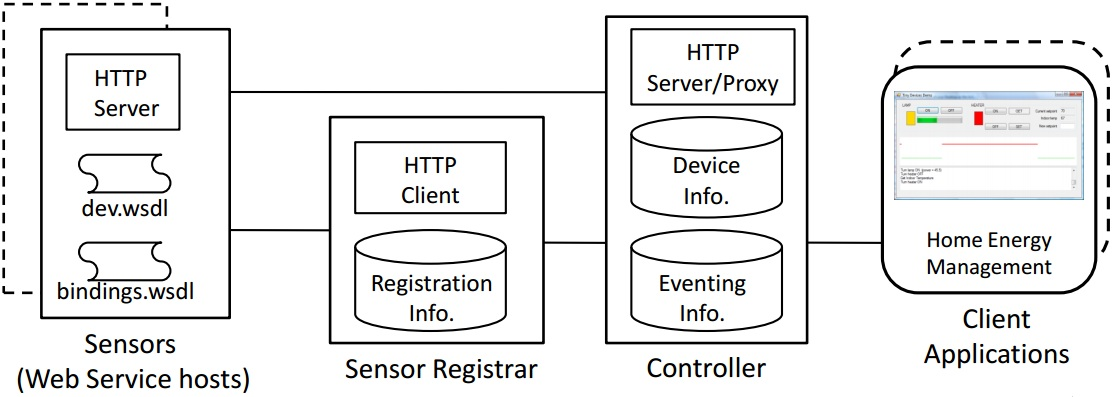
\includegraphics[scale=0.36]{figures/implementation.jpg}
  \caption{Diagramme d'implémentation du service web}
 \end{figure} 
\end{frame}

\begin{frame}
 \frametitle{Implémentation}
 \framesubtitle{Capteurs}
 Chaque capteur contient deux fichiers WSDL:
 \begin{enumerate}
  \item \textbf{\texttt{dev.wsdl}} Décrit complètement les méthodes supportées par le capteur et accessibles pour l'utilisateur. Noms de méthodes avec leurs paramètres, type des paramètres et de la valeur retournée.
  \item \textbf{\texttt{bindigs.wsdl}} Importe \texttt{dev.wsdl} et ajoute 3 méthodes accessibles seulement pour le controleur:
   \begin{enumerate}
    \item \texttt{void eventOn(string eventName)}
    \item \texttt{void eventOff(string eventName)}
    \item \texttt{void setHandlerURL(string url)}
   \end{enumerate}
   Pour autoriser à poster l'évenement \texttt{eventName} à l'adresse URL \texttt{url}
 \end{enumerate}
 Le capteur lance un serveur HTTP qui accède au fichier \texttt{bindigs.wsd}.\\
 La requête est encodée dans l'URL et retourne un fichier XML.
\end{frame}

\begin{frame}
 \frametitle{Implémentation}
 pour ajouter un nouveau capteur dans le réseau, l'\textit{enregistreur} (Sensor Registrar) télécharge les fichiers wsdl et enregistres les données dans un fichier XML avec une IP préétablie et un nom donné par l'utilisateur.
 Ensuite il envoie le XML au controleur.
 Il peut être implémenté aussi bien dans un PC qu'un point d'accès 802.15.4.\\
 \vspace{4mm}
 Le \textit{controleur} agit comme un serveur HTTP.
 \begin{exampleblock}{Exemples de requête}
 \begin{itemize}
  \item \texttt{http://Controller/index.htm}\\retourne la liste des capteurs enregistrés.
  \item \texttt{http://Controller/wsdl/<sensorName>.wsdl}\\retourne la description WSDL du capteur \texttt{<sensorName>}
 \end{itemize} 
 \end{exampleblock}
\end{frame}


\newcommand{\unite}{(octets)}
\begin{frame}%[fragile]
 \frametitle{Implémentation}
 \framesubtitle{Mémoire utilisée}
 \begin{center}
 \begin{tabular}{|l|r|r|r|}
  \hline
  Module & Code & Data & Const\footnote{\textbf{Const}: Constantes enregistrées dans la ROM}\\
  ~ & \unite & \unite & \unite \\
  \hline
  Librairies & 804 & 2 & 76\\
  controle hardware & 408 & 78 & 12\\
  Driver radio & 4282 & 404 & 14\\
  TCP/IP & 2964 & 332 & 4\\
  Serveur web+parseur XML & 2380 & 54 & 4864\\
  \hline
  \textbf{Total} & \textbf{10838} & \textbf{870} & \textbf{4970}\\
  \hline
 \end{tabular}
 \end{center}
\end{frame}

\begin{frame}
 \frametitle{Résultats}
 %Grâce à un algorithme qui baisse la température du chauffage lorsque la maison est innocupée, ils ont pu économiser 7,2\% d'énergie de chauffage.\\
 Économie totale d'énergie par jour:
 \begin{figure}
  \centering
  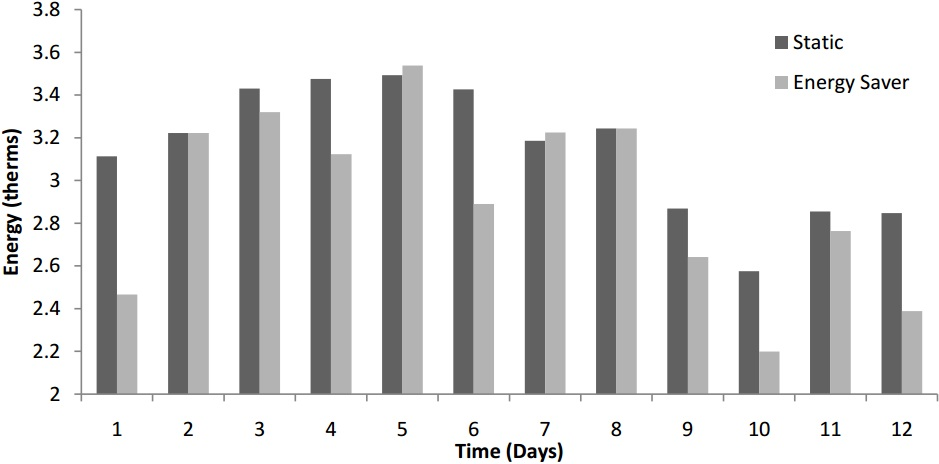
\includegraphics[scale=0.38]{figures/energysaver.jpg}
  \caption{Économie d'énergie totale}
 \end{figure} 
\end{frame}

 
 
